\chapter{Design von Rayden}
\label{cha:Design}

Im vorigen Kapitel wurde der Ablauf eines Testprojekts aufgezeigt und eine Einführung in das Thema \enword{Keyword-Driven Testing} gegeben. In diesem Kapitel wird das Rayden-System detailliert erklärt. Zu Beginn werden die Designziele der Sprache Rayden erklärt. Die Sprache Rayden ist eine domänenspezifische Sprache, welche einige Eigenheiten und Überraschungen enthält. In den weiteren Abschnitten wird der Aufbau des Rayden-Systems erklärt und auf die technischen Details eingegangen. Am Ende dieses Kapitels wird noch die Integration in die \enword{Java-Scripting-API} \cite{JavaScriptApi} beschrieben. Das Rayden-System bietet die Möglichkeit, dass man einen Test in einer Java-Anwendung über das \enword{Java-Scripting-API} ausführen kann.

%%------------------------------------------------------------------------------------------------------

\section{Designziele von Rayden}

Das primäre Designziel von Rayden ist Offenheit. Rayden soll im gesamten Testprozess einsetzbar sein, darf aber die involvierten Personen nicht überfordern. Um dieses Ziel zu erreichen, setzt das Rayden-System auf mehreren Ebenen an.

\SuperPar
Die domänenspezifische Sprache von Rayden ist speziell für Personen im Testbereich ausgelegt. Das wichtigste Ziel der Sprache ist Einfachheit. Die Sprache soll Personen ohne Programmierkenntnisse in die Lage versetzen, Tests in dieser Sprache zu lesen und zu bearbeiten. Die Sprache Rayden ist daher stark an der natürlichen Sprache angelehnt, um den Einstieg zu erleichtern. Ein anderes Ziel bei dem Sprachdesign ist die Flexibilität der Sprache. Der Testprozess setzt sich aus einer Vielzahl an unterschiedlichen Aufgaben zusammen. Um möglichst alle Aufgaben mit dieser Sprache abdecken zu können, wird eine hohe Flexibilität benötigt. 

\SuperPar
Abgesehen von einer geeigneten Sprache gibt es noch weitere wichtige Ziele für das Rayden-System. Rayden muss plattformunabhängig sein, um viele Anwendungsszenarien abdecken zu können. Aus diesem Grund wird die Programmiersprache \enword{Java} für die Entwicklung des Rayden-Systems gewählt. Der Interpreter für Rayden selbst läuft auch wieder auf der virtuellen \enword{Java}-Maschine (JVM).

\SuperPar
Die Einbindung von externen Test-Treiber-Bibliotheken wird durch eine offene Schnittstelle ermöglicht. Dadurch können mit Rayden-Tests für die unterschiedlichsten Anwendungsszenarien entwickelt werden. Rayden kann somit für das jeweilige Projekt und die beteiligten Personen angepasst werden. 

%%------------------------------------------------------------------------------------------------------

\section{Aufbau des Rayden-Systems}

In diesem Abschnitt wird der Aufbau des Rayden-Systems von zwei Blickwinkeln aus beleuchtet. Zuerst wird der konzeptionelle Aufbau erklärt. Dabei wird darauf eingegangen, wie die einzelnen Konzeptebenen miteinander kommunizieren und welche Person für die jeweilige Ebene verantwortlich ist. Im zweiten Teil wird die technische Architektur des Rayden-Systems erläutert. Dazu werden die Komponenten und ihre Beziehungen überblicksweise erklärt. Eine ausführliche Beschreibung findet man in den Abschnitten \ref{cha:KonzeptAufbau} und \ref{cha:TechArch}.

\subsection{Konzeptioneller Aufbau}
\label{cha:KonzeptAufbau}

Wie schon in vorigen Abschnitten erwähnt, ist Rayden an das Konzept von \enword{Keyword-Driven Testing} angelehnt. Bevor der Aufbau von Rayden beschrieben wird, wird der konzeptionelle Aufbau von \enword{Keyword-Driven Testing} erläutert. 

\begin{figure}[h]
\centering
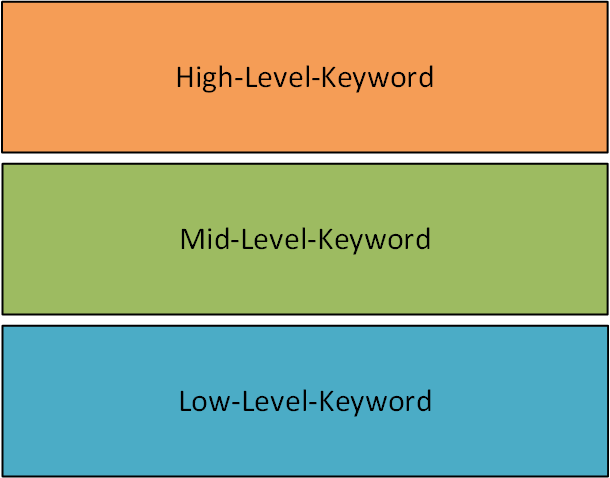
\includegraphics[width=0.7\textwidth]{KDT-Architektur.png}
\caption{Aufbau von \enword{Keyword-Driven Testing}}
\label{fig:kdt-arch}
\end{figure}

\SuperPar
Ein \enword{Keyword-Driven}-Test besteht aus einer Sequenz von \enword{Keywords}. Diese \enword{Keywords} können wiederum aus einer Sequenz von \enword{Keywords} bestehen oder mit einem Codestück verbunden sein. Die \enword{Keywords} werden in drei Kategorien, wie in Abbildung \ref{fig:kdt-arch} dargestellt, aufgeteilt. Die \enword{High-Level Keywords} repräsentieren einen Testfall mit einer detaillierten Beschreibung. Diese Gruppe von \enword{Keywords} wird typischerweise von einer Person aus der Fachabteilung oder von einer Testmanagerin oder einem Testmanager erstellt. Dabei wird aber nur der Rumpf des \enword{Keywords} erstellt. Die Implementierung wird erst in der nächsten Phase hinzugefügt. Diese \enword{High-Level Keywords} bilden die Grundlage für die Erstellung der Tests. In der weiteren Phase werden diese \enword{Keywords} von Testerinnen und Testern implementiert.

\SuperPar
Die \enword{High-Level Keywords} bestehen typischerweise aus einer Sequenz von \enword{Mid-Level Keywords}. Diese Sequenz wird in der zweiten Phase erstellt. Normalerweise finden sich \enword{Mid-Level Keywords} in dieser Sequenz, es können aber auch \enword{Low-Level Keywords} verwendet werden. Die verwendeten \enword{Mid-Level Keywords} bestehen wiederum aus einer Sequenz von \enword{Mid-Level Keywords} und \enword{Low-Level Keywords}. Technisch gesehen gibt es keinen Unterschied zwischen \enword{High-Level Keywords} und \enword{Mid-Level Keywords}. Der Unterschied besteht nur in der Art der Verwendung. \enword{High-Level Keywords} beschreiben genau einen Anwendungsfall der getestet werden soll. Im Gegenteil zu \enword{Mid-Level Keywords} wird hier kein Wert auf Wiederverwendung gelegt.

\SuperPar
In der letzten Phase werden \enword{Low-Level Keywords} mit Code verbunden. Der Code kann prinzipiell in jeder Programmiersprache geschrieben sein. Die Wahl der Programmiersprache hängt von dem verwendeten \enword{Keyword-Driven Framework} ab. In diesen \enword{Keyword-Driven Frameworks} werden häufig Skript-Sprachen verwendet. Der Vorteil von Skript-Sprachen liegt darin, dass der Code für die Ausführung des Tests nicht kompiliert werden muss.

\begin{figure}[h]
\centering
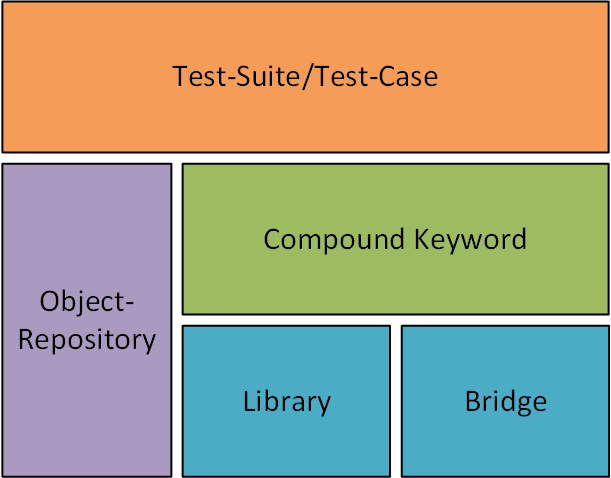
\includegraphics[width=0.7\textwidth]{Rayden-Architektur.png}
\caption{Aufbau von Rayden}
\label{fig:rayden-arch}
\end{figure}

\SuperPar
Im Gegensatz zu \enword{Keyword-Driven Testing} unterteilt das Rayden-System die \enword{Keywords} in mehr Gruppen, wie in Abbildung \ref{fig:rayden-arch} dargestellt. Die zusätzlichen Gruppen bieten einen bessere Strukturierung und geben eine klare Richtung vor, wie ein Rayden-Test-Projekt aufgebaut werden soll.    

\SuperPar
Rayden führt eine klare Trennung bei \enword{Low-Level Keywords} ein. Diese \enword{Keywords}, welche mit einem Codestück verbunden sind, werden in \enword{Library-} und \enword{Bridge-Keywords} unterteilt. \enword{Library-Keywords} stellen grundlegende Funktionen bereit, welche unabhängig von einem speziellen Anwendungsfall sind. Als Beispiel kann man sich eine \enword{For}- oder \enword{Print-Keyword} vorstellen. Im Gegensatz dazu sind \enword{Bridge-Keywords} speziell für eine Anwendungstechnologie angepasst, wie zum Beispiel \enword{Open Browser} oder \enword{Navigate To} für Web-Anwendungen. 

\SuperPar
Auch bei den \enword{High-Level Keywords} bietet Rayden eine größere Vielfalt. Grob werden diese in Test-Suiten und Testfälle unterteilt. Die Test-Suite dient als Gruppierungselement für Testfälle, um diese gemeinsam ausführen zu können. Bei der Definition von Testfällen können diese mit unterschiedlichen Testtypen angelegt werden. Eine nähere Beschreibung findet sich im Abschnitt \ref{cha:KeywordTypes}.

\SuperPar
Zum Abschluss ist noch auf das \enword{Object Repository} hinzuweisen. Diese Komponente verwaltet Test-Objekte. Test-Objekte können für die Beschreibung von Benutzeroberflächen-Komponenten wie Schaltflächen oder Eingabefelder verwendet werden. Dafür wird für jedes Test-Objekt ein Bezeichner definiert, mit welchem man die Komponente in der Benutzeroberfläche finden kann. Das ist im Fall einer Web-Anwendung ein \enword{XPath}- oder ein \enword{CSS}-Ausdruck. Das \enword{Object Repository} sorgt somit für eine klare Trennung zwischen Test- und Benutzeroberflächen-Beschreibung. Diese Trennung erhöht die Wiederverwendbarkeit von \enword{Keywords} und reduziert den Wartungsaufwand bei Änderungen an der Benutzerschnittstelle.

\subsection{Technische Architektur}
\label{cha:TechArch}

Die technische Basis für das Rayden-System ist die \enword{Java}-Plattform. Auf der Entwicklungsseite wird \enword{Java} als Programmiersprache für das gesamte Rayden-System verwendet, auf der Ausführungsseite läuft das Rayden-System auf der virtuellen Java-Maschine (JVM). Außerdem bietet Rayden die Möglichkeit, dass man einen Rayden-Test über das \enword{Java Scripting API} \cite{JavaScriptApi} ausführen kann. 

\begin{figure}[h]
\centering
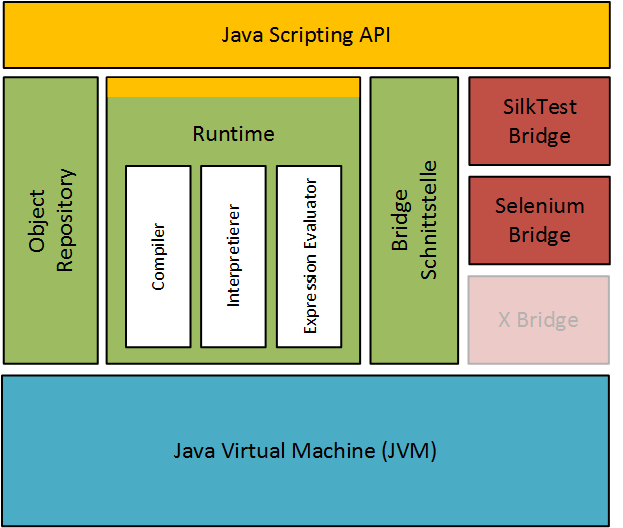
\includegraphics[width=0.9\textwidth]{Rayden-Tech-Architektur.png}
\caption{Rayden-Architektur}
\label{fig:rayden-tech-arch}
\end{figure}

\SuperPar
Abbildung \ref{fig:rayden-tech-arch} zeigt alle Komponenten des Rayden-Kernsystems in Grün. Diese Komponenten bilden die Grundlage dafür, einen Rayden-Test ausführen zu können. Als Basis dieser Komponenten sieht man in Blau die virtuelle Java-Maschine (JVM). Die externen \enword{Bridge}-Implementierungen werden in Rot dargestellt. Diese Komponenten stellen eine Verbindung zwischen dem Test-Treiber und der Rayden-\enword{Runtime} her und werden über die \enword{Bridge}-Schnittstelle hergestellt. Im oberem Abschnitt der Abbildung \ref{fig:rayden-tech-arch} sieht man das \enword{Java Scripting API}, über welches man Rayden-Tests ausführen kann.

\SuperPar
Im nächsten Absatz werden die einzelnen Komponenten der Rayden-Architektur beschrieben, um einen groben Überblick über die Funktionsweise von Rayden zu geben.\\

\begin{itemize}

\item \textbf{Runtime}

Die \enword{Runtime} ist der Einstiegspunkt für die Ausführung von Rayden-Tests. Dazu enthält diese Komponente die Implementierung für die \enword{Java Scripting API}. Wird ein Test ausgeführt, werden zuerst alle Projektressourcen in der \enword{Runtime} geladen. Das Projektverzeichnis kann man über einen Kontextparameter setzen. Falls dieser nicht gesetzt ist, wird das aktuelle Verzeichnis verwendet. Für das Laden der Ressourcen wird die Compiler-Komponente verwendet. Die \enword{Runtime} baut bei diesem Lesevorgang eine \enword{Lookup}-Tabelle für alle \enword{Keywords} auf. Diese Tabelle wird für einen schnellen Zugriff im Interpreter benötigt. Der Rayden-Test wird mithilfe des Interpreters ausgeführt. Das Ergebnis des Tests wird als Resultat über die \enword{Java Scripting API} zurückgegeben.\\

\item \textbf{Compiler}

Der Compiler für die Rayden-Sprache wird mit dem Compiler-Werkzeug xText \cite{xtext} realisiert. Von dem generierten Compiler wird für die Ausführungseinheit nur der lexikalische und syntaktische Analysator verwendet. Der Eclipse-Editor wird für das Rayden-System nicht benötigt. Das Resultat der Compiler-Komponente ist ein EMF-Modell des Tests. Die \enword{Runtime}-Komponente verwaltet die Modelle und stellt diese dem Interpreter bei Bedarf zur Verfügung.\\

\item \textbf{Interpreter}

Der Interpreter ist die wichtigste Komponente im Rayden-System. Der Interpreter ist dafür verantwortlich, dass die Rayden-Tests ausgeführt werden können. Zum Starten des Interpreters wird der Aufruf eines \enword{Test-Keywords} übergeben. Dieses \enword{Keyword} wird auf den leeren \enword{Stack} geladen. Der Test wird mithilfe einer \enword{Stack}-Maschine \cite{StackMachine} abgearbeitet. Bei jedem Aufruf eines \enword{Keywords} wird die \enword{Keyword}-Implementierung auf den \enword{Stack} geladen. Zusätzlich wird für jeden neuen \enword{Keyword}-Aufruf ein neuer Gültigkeitsbereich (\enword{Scope}) angelegt. \\
\\
Der Gültigkeitsbereich ist für die Verwaltung der Parameter und Variablen zuständig. Eine Besonderheit in Rayden ist, dass Gültigkeitsbereiche Zugriff auf andere Gültigkeitsbereiche haben. Eine detaillierte Beschreibung dazu findet sich im Abschnitt \ref{cha:KeywordScope}. Die Auswertung von Ausdrücken wird in einem separaten Teil des Interpreters vorgenommen. Für die Auswertung wird der aktuelle Gültigkeitsbereich und der Ausschnitt aus dem Modell an die Evaluierungskomponente übergeben. Das Ergebnis des Ausdrucks wird wieder auf den \enword{Stack} gelegt. Ruft die \enword{Stack}-Maschine ein \enword{Scripted-Keyword} (Beschreibung in Abschnitt \ref{cha:Keyword}) auf, wird entweder der dazugehörige Code ausgeführt oder es wird der Aufruf an die \enword{Bridge}-Schnittstelle weitergeleitet.\\

\item \textbf{Bridge-Schnittstelle}

Die \enword{Bridge}-Schnittstelle ist für die Anbindung von Test-Treibern verantwortlich. Um einen Test-Treiber verwenden zu können, muss eine Rayden-\enword{Bridge} implementiert werden. Die \enword{Bridge} mit der Schnittstelle bildet die Verbindung zwischen der Rayden-\enword{Runtime} und dem Test-Treiber.\\

\item \textbf{Object-Repository}

Das \enword{Object Repository} verwaltet Test-Objekte, welche von \enword{Keywords} verwendet werden können. Die Test-Objekte werden in einer Baumstruktur verwaltet. Die wichtigste Eigenschaft eines Test-Objekts ist der Bezeichner (\enword{Locator}). Mit dem Bezeichner kann die Benutzerschnittstellen-Komponente identifiziert werden. Das Konzept ist an der Idee von \enword{Page-Object-Pattern} \cite{PageObject} angelehnt. \\

\end{itemize}


%%------------------------------------------------------------------------------------------------------

\section{Sprache von Rayden}

Als Inspiration und Basis für die Sprache dient das Konzept von \enword{Keyword-Driven Testing}. Das Grundprinzip hinter \enword{Keyword-Driven Testing} ist die Verwendung von \enword{Keywords}. Ein \enword{Keyword} besteht aus einer Sequenz von anderen \enword{Keywords} oder ist mit einem Codestück verbunden. Einen \enword{Keyword-Driven}-Test kann man sich auch als gerichteten Graph vorstellen, in dem die Knoten die \enword{Keywords} repräsentieren und die Kanten die Abhängigkeit zwischen den \enword{Keywords} beschreiben, wie in Abbildung \ref{fig:test-graph} dargestellt.

\begin{figure}[h]
\centering
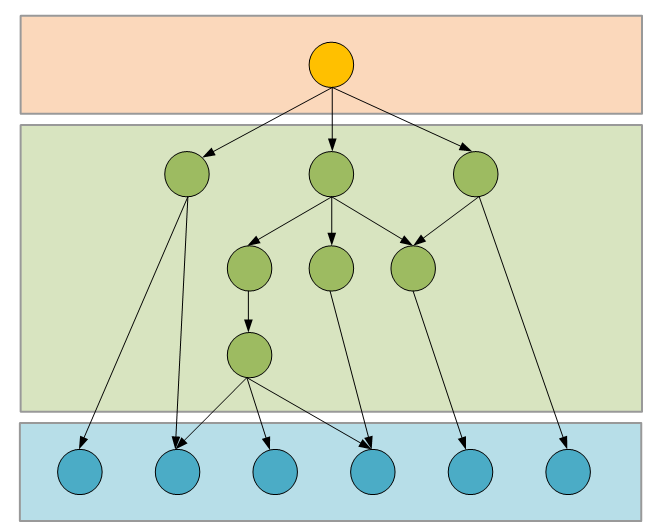
\includegraphics[width=0.8\textwidth]{Rayden-Testbaum.png}
\caption{Graph-Repräsentation eines Tests}
\label{fig:test-graph}
\end{figure}

\SuperPar
Der gelbe Knoten repräsentiert ein \enword{High-Level Keyword}. Von diesem Knoten aus werden über gerichtete Kanten die Beziehungen zu den \enword{Mid-Level Keywords} in Grün definiert. Man sieht, dass die \enword{Mid-Level Keywords} entweder wieder in Beziehungen zu anderen \enword{Mid-Level Keywords} stehen oder \enword{Low-Level Keywords} referenzieren. Die \enword{Low-Level Keywords} werden in Blau dargestellt. Bei den Graphen handelt es um einen gerichteten azyklischen Graph (DAG).

\SuperPar
Die Rayden-Sprache setzt auch auf dieses Konzept von \enword{Keywords}. Im Unterschied zu \enword{Keyword-Driven Testing} setzt Rayden auf eine größere Vielfalt an unterschiedlichen \enword{Keywords}, welche im nächsten Abschnitt \ref{cha:Keyword} detailliert beschrieben werden. Ein weiterer Unterschied ist die Benennung von \enword{Keywords}. Normalerweise besteht der Name eines \enword{Keywords} nur aus einem Wort, damit die Verarbeitung der Tests für den Compiler erleichtert wird. In der Rayden-Sprache wird ein großes Augenmerk darauf gelegt, dass man nicht nur auf ein Wort beschränkt ist, sondern auch ganze Sätze als Namen verwenden kann. Diese Eigenschaft ist sehr nützlich, um die Testfälle wie in einer natürlichen Sprache beschreiben zu können. Der Vorteil ist, dass man somit ohne weiteren Aufwand eine ordentliche Dokumentation des Tests bekommt.

\SuperPar
Eine andere interessante Eigenschaft der Sprache ist, dass in der Sprache keine Sprung-Operationen enthalten sind. Die Konsequenz daraus ist, dass es in der Sprache auch keine Schleifen- oder Verzweigungs-Konstrukte enthalten sind. Die einzige Möglichkeit, um ähnliche Konstrukte zur Verfügung zu stellen, sind \enword{Scripted Compound Keywords}, wobei man bei diesem Metatyp von \enword{Keyword} auch nur entscheiden kann, ob eine Sequenz von \enword{Keywords} ausgeführt werden soll. Das Konzept der Metatypen wird im Abschnitt \ref{cha:Keyword} beschrieben. 

\SuperPar
Da Sprung-Operationen vermieden werden und die Sprache blockstrukturiert ist, gewinnt man die Fähigkeit, Tests visuell darstellen zu können. Diese Fähigkeit ist hilfreich, um eine bessere Unterstützung und einen leichteren Einstieg in die Sprache zu ermöglichen. Das ist vor allem von Vorteil, wenn Personen aus einer Fachabteilung nur unregelmäßig damit arbeiten müssen. 

%%------------------------------------------------------------------------------------------------------

\section{\enword{Keywords} von Rayden}
\label{cha:Keyword}

Das \enword{Keyword} ist die Schlüsselkomponente der Sprache Rayden. In diesem Abschnitt werden die unterschiedlichen Typen und Metatypen erklärt und gezeigt, wofür diese verwendet werden können. Am Anfang werden die vier Metatypen von \enword{Keywords} erklärt. Die Metatypen sind die Basis für den Funktionsumfang der Sprache. Ferner werden die unterstützten Typen beschrieben und wofür diese verwendet werden können. Als Abschluss werden noch Themen wie Sichtbarkeit, Benennung und Parameter erläutert.

%%------------------------------------------------------------------------------------------------------

\subsection{Metatypen}

Der Metatyp definiert die Funktionsweise eines \enword{Keywords}. Rayden unterscheidet zwischen vier Metatypen, wobei einer dieser Metatypen nur eine Kurzform ist.

%%------------------------------------------------------------------------------------------------------

\subsection{Metatyp: \enword{Compound Keyword}}

Das \enword{Compound Keyword} ist die einfachste Variante eines \enword{Keywords}. Bei einem \enword{Compound Keyword} wird eine Sequenz von \enword{Keywords} zu einem neuen \enword{Keyword} zusammengefasst. Der Beispiel-Code \ref{prog:compoundKeyword} zeigt die Verwendung eines \enword{Compound Keywords}. In dem Beispiel kann man gut sehen, dass dieser Metatyp hauptsächlich für die Strukturierung von Tests verwendet wird. Ein mögliches Vorgehen kann dabei sein, dass man einen Testfall immer weiter und weiter in \enword{Keywords} zerlegt, bis man am Ende die Aufgabe auf einzelne Aktionen heruntergebrochen hat. Für diese Aktionen werden dann \enword{Scripted Keywords} verwendet wie im Code-Beispiel die beiden \enword{Keywords} \enword{Type Text} und \enword{Click Left}.

\begin{program}
\begin{JavaCode}
keyword Anmelden an der PetClinic Anwendung {
	'''Man meldet sich bei der Anwendung PetClinic mit den definierten 
	   Daten an. Wenn das Keyword erfolgreich ausgeführt worden ist, 
	   befindet man sich auf der Hauptseite der Webanwendung.'''
	
	parameter in username as string
	parameter in password as string
	
	Type Text(@PetClinic.LoginPage.Username, username)
	Type Text(@PetClinic.LoginPage.Password, password)
	
	Click Left(@PetClinic.LoginPage.LoginButton)
}
\end{JavaCode}
\caption{Das Beispiel zeigt das \enword{Compound Keyword} Anmelden an der PetClinic Anwendung}
\label{prog:compoundKeyword}
\end{program}

\SuperPar
Ein klares Ziel bei der Erstellung von \enword{Compound Keywords} ist die Wiederverwendung. Ein \enword{Compound Keyword} soll als eine logische Einheit aufgebaut werden, sodass man diese auch wieder für andere Tests verwenden kann. 

%%------------------------------------------------------------------------------------------------------

\subsection{Metatyp: \enword{Inline Keyword}}

Der Metatyp \enword{Inline Keyword} ist eine Kurzform des \enword{Compound Keywords}. Dabei kann man in einem \enword{Compound Keyword} ein neues \enword{Keyword} erstellen. Daher kommt auch der Name \enword{Inline Keyword}, weil es innerhalb eines anderen \enword{Keywords} erstellt wird. Im Beispiel \ref{prog:inlineKeyword} wird im \enword{Keyword} \enword{Anmelden an der PetClinic Anwendung} das \enword{Inline Keyword} \enword{Besitzer anlegen} definiert. Es werden alle Schritte zum Anlegen eines neuen Besitzers zusammengefasst. Der Anwendungsfall dieses Metatyps ist wiederum die Strukturierung, aber in diesem Fall innerhalb eines \enword{Keywords}. 

\begin{program}
\begin{JavaCode}
testcase Anlegen eines neuen Besitzers {
	'''Der Testfall überprüft den Anwendungsfall um einen 
	   neuen Besitzer anlegen zu können.'''
	
	Anmelden an der PetClinic Anwendung ("max", "secret")
	
	Besitzer anlegen {
		Oeffnen der Besitzerseite		
		Neuen Besitzer in der Anwendung anlegen("Huber", "Mayr")
		Daten von Besitzer ueberpruefen
	}
	
	Abmelden von der Anwendung
}
\end{JavaCode}
\caption{Beispiel von einem \enword{Inline Keyword}}
\label{prog:inlineKeyword}
\end{program}

\SuperPar
Der Nachteil bei dieser Variante ist, dass man dieses \enword{Keyword} nicht wiederverwenden kann. Das \enword{Inline Keyword} ist nur innerhalb des \enword{Compound Keywords} bekannt.

%%------------------------------------------------------------------------------------------------------

\subsection{Metatyp: \enword{Scripted Keyword}}

Das \enword{Scripted Keyword} ist der einfachere Metatyp, mit welchem man Code an ein \enword{Keyword} binden kann. Ein \enword{Scripted Keyword} wird wie ein \enword{Compound Keyword} definiert. Im Unterschied dazu besitzt das \enword{Scripted Keyword} keine Sequenz von \enword{Keywords}, sondern einen Hinweis auf die Implementierung. Im Beispiel-Code \ref{prog:scriptedKeyword} sieht man eine Variante mit einer \enword{Java}-Implementierung. Die Anweisung \enword{implemented in java} definiert die Implementierungssprache. Nach dem Pfeil folgt ein Bezeichner, welcher die Implementierung referenziert. Im Fall von \enword{Java} wird der vollständige Name der Klasse verwendet.

\begin{program}
\begin{JavaCode}
keyword Print {
	'''Der Parameter 'text' wird in den Test-Report geschrieben.'''
	
	parameter text
	implemented in java -> "com.github.thomasfischl.rayden.runtime.keywords.impl.PrintKeyword"
}
\end{JavaCode}
\caption{Rayden: Beispiel \enword{Scripted Keyword}}
\label{prog:scriptedKeyword}
\end{program}

\SuperPar
Um die \enword{Java}-Klasse als \enword{Keyword}-Implementierung verwenden zu können, muss die Klasse das \enword{Interface} \enword{ScriptedKeyword} implementieren. Das \enword{Interface} hat nur die Methode \enword{execute}. Kommt die \enword{Stack}-Maschine zu einem Aufruf eines \enword{Scripted Keywords}, wird ein neues Objekt der \enword{Keyword}-Implementierung über den \enword{Java-Reflection}-Mechanismus angelegt. Von dem Objekt wird dann die Methode \enword{execute} mit dem Namen des aktuellen \enword{Keywords}, dem Gültigkeitsbereich und einem \enword{Reporter}-Objekt aufgerufen. Auf die Parameter des \enword{Keywords} kann man über den Gültigkeitsbereich zugreifen, wie man im Beispiel-Code \ref{prog:scriptedKeywordImpl} sehen kann. Als Ergebnis liefert die Methode ein \enword{KeywordResult}-Objekt. Dieses Objekt signalisiert der \enword{Stack}-Maschine, ob das \enword{Keyword} erfolgreich ausgeführt worden ist.   

\begin{program}
\begin{JavaCode}
public class PrintKeyword implements ScriptedKeyword {

	@Override
	public KeywordResult execute(String keyword, 
			IKeywordScope scope, IRaydenReporter reporter) {
		reporter.log(scope.getVariable("text").toString());
		return new KeywordResult(true);
	}
}
\end{JavaCode}
\caption{Rayden: \enword{Java}-Implementierung des \enword{Print Keywords}}
\label{prog:scriptedKeywordImpl}
\end{program}

\SuperPar
Der Parameter \enword{keyword} bei der Methode \enword{execute} wird benötigt, weil es in Rayden möglich ist, eine Implementierung an mehrere \enword{Keyword}-Definitionen zu binden. Mit diesem Parameter kann man den Namen der aktuellen \enword{Keyword}-Definition abfragen.

\SuperPar
Über das \enword{Reporter}-Objekt kann man Einträge in den Test-Report hinzufügen. Die Instanz bietet unterschiedliche Granularitätsstufen für Nachrichten. Es werden spezielle Methoden für die Stufen Fehler, Warnung und Information angeboten. Diese Nachrichten können in der Folge von den jeweiligen \enword{Reporter}-Implementierungen unterschiedlich behandelt werden. 

%%------------------------------------------------------------------------------------------------------

\subsection{Metatyp: \enword{Scripted Compound Keyword}}

Das \enword{Scripted Compound Keyword} ist die komplizierteste Variante der vier Metatypen, jedoch ist diese Variante essentiell für die Flexibilität der Sprache. Mit dem Konzept von \enword{Scripted Compound Keywords} ist eine Entwicklerin oder ein Entwickler in der Lage, die Sprache um Kontrollstrukturen zu erweitern. Dafür werden die Eigenschaften von \enword{Compound Keywords} und \enword{Scripted Keywords} kombiniert. 

\begin{program}
\begin{JavaCode}
keyword IF { 
	parameter in condition as boolean
	implemented in java -> "com.github.thomasfischl.rayden.runtime.keywords.impl.IfKeyword"
}
\end{JavaCode}
\caption{Beispiel für ein \enword{Scripted Compound Keyword}}
\label{prog:ifKeyword}
\end{program}

\SuperPar
Das \enword{Scripted Compound Keyword} ist mit einem Codestück verbunden und hat zusätzlich noch eine \enword{Keyword}-Liste. In der Implementierung hat man die Möglichkeit, die Ausführung der \enword{Keyword}-Liste zu steuern. Man kann damit eine bedingte bzw. mehrmalige Ausführung der Liste realisieren. Es ist aber zu beachten, dass man die Liste nur als Ganzes steuern kann. Eine teilweise Ausführung der Liste ist nicht möglich.

\SuperPar
Das Beispiel \ref{prog:ifKeyword} zeigt die Definition für ein \enword{IF Keyword}. Dabei wird wie bei einem \enword{Scripted Keyword} die Programmiersprache und der Bezeichner definiert. Im Fall von einem \enword{Scripted Compound Keyword} muss die Klasse das \enword{Interface} \enword{ScriptedCompoundKeyword} implementieren. Dieses \enword{Interface} ist deutlich schwieriger zu implementieren, wie man im Beispiel-Code \ref{prog:ifKeywordImpl} sehen kann.

\begin{program}
\begin{JavaCode}
public class IfKeyword implements ScriptedCompoundKeyword {

  private IKeywordScope scope;

  @Override
  public void initializeKeyword(String keyword, IKeywordScope scope, IRaydenReporter reporter) {
    this.scope = scope;
  }

  @Override
  public boolean executeBefore() {
    return scope.getVariableAsBoolean("condition");
  }

  @Override
  public boolean executeAfter() {
    return false;
  }
  
  @Override
  public KeywordResult finalizeKeyword() {
    return new KeywordResult(true);
  }
}
\end{JavaCode}
\caption{\enword{Java}-Implementierung des \enword{IF Keywords}}
\label{prog:ifKeywordImpl}
\end{program}

\SuperPar
Das \enword{Interface} enthält für jede der vier Phasen eines \enword{Scripted Compound Keywords} eine Methode, in der man die Ausführung steuern kann. \\

\begin{itemize}

\item \textbf{Phase 1: Initialisierung (\enword{initializeKeyword})}\\
In der Initialisierungsphase wird der aktuelle Zustand von der \enword{Stack}-Maschine an die \enword{Keyword}-Implementierung übergeben. Falls die Informationen für die Ausführung benötigt werden, können diese im Objekt gespeichert werden. Eine Instanz der \enword{Keyword}-Implementierung wird genau für eine Ausführung verwendet. Das heißt, man kann keinen globalen Zustand für zukünftige Ausführungen speichern. Falls man diese Funktionalität benötigt, muss man diese Daten in Klassenvariablen speichern.\\

\item \textbf{Phase 2: Beginn der Auswertung (\enword{executeBefore})}\\
Die Ausführung der \enword{Keyword}-Liste kann in dieser Phase beeinflusst werden. Diese Methode wird vor jeder Auswertung der \enword{Keyword}-Liste aufgerufen. Wenn diese Methode \enword{false} liefert, wird die Liste nicht ausgewertet und es wird zur Phase 4 gesprungen.\\

\item \textbf{Phase 3: Beendigung der Auswertung (\enword{executeAfter})}\\
Nach der Ausführung der \enword{Keyword}-Liste wird die Methode \enword{executeAfter} aufgerufen. In dieser Phase wird entschieden, ob die Liste ein weiteres Mal ausgeführt werden soll. Wenn die Methode in dieser Phase \enword{true} liefert, wird die Ausführung bei der zweiten Phase fortgesetzt. Ansonsten wird die vierte Phase ausgeführt.\\

\item \textbf{Phase 4: Beendigung des Keywords (\enword{finalizeKeyword})}\\
In der letzten Phase können noch Abschlussarbeiten vorgenommen werden, wie beispielsweise die Berechnung des Status für das \enword{Keyword}. Der Status signalisiert, ob die Ausführung erfolgreich war oder nicht. Diese Funktionalität kann für Validierungen verwendet werden.

\end{itemize}

\SuperPar
Die Verwendung eines \enword{Scripted Compound Keyword} sieht wie ein \enword{Inline Keyword} aus. Der große Unterschied ist, dass ein \enword{Inline Keyword} keine Parametersignatur im Gegensatz zu einem \enword{Scripted Compound Keyword} hat. Ein Beispiel für die Verwendung findet man im Code-Ausschnitt \ref{prog:ifKeywordUsage}.

\begin{program}
\begin{JavaCode}
keyword If Keyword Bespiel {
	If (a == 1) {
		Print("Condition is true")
	}
	If (test == "b") {
		Print("Condition is false")
	}
}
\end{JavaCode}
\caption{Verwendung des \enword{IF Keywords}}
\label{prog:ifKeywordUsage}
\end{program}

%%------------------------------------------------------------------------------------------------------
\subsection{Typen}
\label{cha:KeywordTypes}

Neben den Metatypen für \enword{Keywords} gibt es in Rayden auch unterschiedliche Typen von \enword{Keywords}. Die Typen liefern keine zusätzliche Funktionalität für die Sprache, sondern dienen als Strukturierungselement für Testprojekte. Mithilfe der Typen kann man Testfälle unterscheiden und eine klare Zuordnung zu einer Testmethode treffen. Durch die Typen wird es auch möglich, eine Aussage über die Verteilung der Testmethoden in einem Testprojekt treffen zu können. 

\SuperPar
Rayden unterstützt die folgenden \enword{Keyword}-Typen:

\begin{itemize}
\item Test-Suite (\enword{TestSuite}),
\item Testfall (\enword{TestCase}),
\item Komponententest (\enword{UnitTest}),
\item Integrationstest (\enword{IntegrationTest}),
\item Schnittstellentest (\enword{APITest}),
\item Automatisierter Abnahme-Test (\enword{AUTest}) und
\item Manueller Abnahme-Test (\enword{MAUTest}).
\end{itemize}

\SuperPar
In Rayden ist es aber nicht zwingend notwendig, diese Typen zu verwenden. Man kann statt den Typen einfach das Schlüsselwort \enword{keyword} verwenden. Damit verliert man aber die Auswertungsmöglichkeit in einem Testprojekt. 

%%------------------------------------------------------------------------------------------------------
\subsection{Gültigkeitsbereich}
\label{cha:KeywordScope}

In Rayden wird für jeden Aufruf eines \enword{Keywords} ein neuer Gültigkeitsbereich angelegt. In diesem Gültigkeitsbereich befinden sich alle Parameter, welche für das \enword{Keyword} definiert sind. Nachdem Parameter in einem Gültigkeitsbereich definiert worden sind, verhalten sich diese gleich wie Variablen. Variablen können von einem \enword{Keyword} in einem Gültigkeitsbereich mit einem Wert belegt werden. Der Wert einer Variablen kann entweder in einem Ausdruck oder in einem \enword{Keyword} verwendet werden. In Rayden müssen Variablen nicht deklariert werden. Sobald das erste Mal eine Variable mit einem Wert belegt worden ist, ist diese im Gültigkeitsbereich vorhanden.

\begin{figure}[h]
\centering
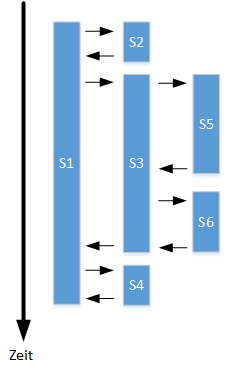
\includegraphics[width=0.5\textwidth]{Rayden-Scope.png}
\caption{Gültigkeitsbereiche in einem Rayden-Test}
\label{fig:rayden-scope}
\end{figure}

\SuperPar
In Rayden gibt es aber noch eine Besonderheit in Bezug auf Gültigkeitsbereiche. Rayden verwendet für die Gültigkeitsbereiche das Konzept von \enword{Dynamic Scoping}. Bei einem Aufruf eines \enword{Keywords} wird der Gültigkeitsbereich mit den Parametern angelegt. Das Besondere ist, dass der neue Gültigkeitsbereich eine Referenz auf den alten Gültigkeitsbereich hat. Das Resultat ist, dass jeder Kind-Gültigkeitsbereich Zugriff auf den Eltern-Gültigkeitsbereich hat.

\SuperPar
Ein Beispiel dazu sieht man in der Abbildung \ref{fig:rayden-scope}. Beim Starten eines Tests wird der Gültigkeitsbereich G1 angelegt. Auf diesen Gültigkeitsbereich haben später alle anderen Gültigkeitsbereiche Zugriff. Daher eignet sich dieser Gültigkeitsbereich gut für globale Variablen.

\SuperPar
In der Abbildung sieht man weiter, dass jeder neue Gültigkeitsbereich eine Beziehung zu einem Eltern-Gültigkeitsbereich hat. Der Pfeil von einem Kind- zu einem Eltern-Gültigkeitsbereich mag am Anfang komisch wirken. Den Pfeil kann man aber damit erklären, dass es in Rayden möglich ist, einen \enword{Out-} bzw. \enword{InOut}-Parameter zu definierten. Damit können Variablen aus G2 an G1 übertragen werden. Eine detaillierte Beschreibung zu den Parametern findet man im Abschnitt \ref{cha:Parameter}.

\SuperPar
Der Vorteil von vererbten Gültigkeitsbereichen ist, dass nicht alle Variablen übergeben werden müssen, welche bei einem Test zahlreich vorkommen können. Die Parameter bieten die Möglichkeit, für eine explizite Definition von Variablen. Das wird verwendet, um sicherzustellen, dass eine Variable definitiv zur Verfügung steht bzw. erleichtert auch die Verwendung eines \enword{Keywords}.

%%------------------------------------------------------------------------------------------------------
%\subsection{Benennung}
%\todo 

%%------------------------------------------------------------------------------------------------------
\subsection{Parameter}
\label{cha:Parameter}

\enword{Keywords} unterstützen das Definieren von Parametern für eine einfachere Verwendung. Grundsätzlich werden Parameter in Rayden nicht zwingend benötigt, da Rayden das Konzept von vererbten Gültigkeitsbereichen verwendet. Parameter ermöglichen jedoch eine explizite Schnittstelle für \enword{Keywords}. 

\begin{program}
\begin{JavaCode}
keyword Parameter Bespiel {
	
	parameter in    parm1
	parameter in    parm2 as string
	parameter out   param3 as boolean
	parameter inout param4 as number
	
	Test1	
}
\end{JavaCode}
\caption{Verwendung von Parametern}
\label{prog:parameter}
\end{program}


\SuperPar
Rayden unterstützt sowohl typisierte als auch untypisierte Parameter. Sind die Parameter typisiert, werden diese vom Rayden-Interpreter überprüft. Sind keine Werte für einen Parameter vorhanden, wird die Ausführung mit einem Fehler abgebrochen. 

\SuperPar
Neben einem Typ kann man bei einem Parameter auch noch die Richtung definieren. Die Richtung bezieht sich auf die Gültigkeitsbereich. In Rayden werden die Richtungen \enword{In}, \enword{Out} und \enword{InOut} unterstützt, wie man im Code-Beispiel \ref{prog:parameter} sehen kann. \\

\begin{itemize}
\item \textbf{\enword{In}-Parameter}\\
Der \enword{In}-Parameter transferiert einen Wert aus dem Eltern-Gültigkeitsbereich in den Kinder-Gültigkeitsbereich. Das ist auch das Standardverhalten, falls keine Richtung bei einem Parameter definiert ist.\\

\item \textbf{\enword{Out}-Parameter}\\
Der \enword{Out}-Parameter ist das genaue Gegenteil zum \enword{In}-Parameter. Dabei wird ein Wert aus dem Kinder-Gültigkeitsbereich in den Eltern-Gültigkeitsbereich transferiert. \\

\item \textbf{\enword{InOut}-Parameter}\\
Der dritte Variante ist eine Kombination aus dem \enword{In}-Parameter und dem \enword{Out}-Parameter.\\
\end{itemize}

%%------------------------------------------------------------------------------------------------------
\section{Datentypen von Rayden}

Die Sprache Rayden unterstützt die folgenden Datentypen:

\begin{itemize}
\item \enword{number},
\item \enword{string},
\item \enword{boolean},
\item \enword{variable},
\item \enword{location} und
\item \enword{enumeration}.
\end{itemize}

\SuperPar
Darunter befinden sich einige Standard-Datentypen wie \enword{number}, \enword{string} und \enword{boolean}. 

\begin{program}
\begin{JavaCode}
keyword Open Browser { 
	parameter in browserType as enumeration (IE | FF | CHROME)

	implemented in java -> "selenium.OpenBrowserKeyword"
}
\end{JavaCode}
\caption{Verwendung von einem \enword{enumeration}-Parameter}
\label{prog:enum}
\end{program}

\SuperPar
Der Typ \enword{enumeration} wird intern als \enword{string} repräsentiert. Die Laufzeitumgebung sorgt dafür, dass nur die vordefinierten Werte zugewiesen werden dürfen. Diese Überprüfung wird aber nur bei einem Übergang von einem Gültigkeitsbereich in einen anderen Gültigkeitsbereich vorgenommen. Diese Einschränkung ist damit zu erklären, dass ein \enword{enumeration}-Datentyp genau für ein \enword{Keyword} definiert wird. Ein Beispiel dazu sieht man im Code-Ausschnitt \ref{prog:enum}.  

\SuperPar
Ein weiterer spezieller Datentyp ist \enword{location}. Mit diesem Datentyp kann man ein Objekt in einem \enword{Object Repository} referenzieren. Ein Wert dieses Datentyps beginnt immer mit einem @-Symbol. Nachfolgend kann man einen Pfad im \enword{Object Repository} beschreiben, wie man im Beispiel \ref{prog:locator} sehen kann. Für Abnahme-Tests ist das Referenzieren von Test-Objekten essentiell. Daher bietet Rayden dafür eine Erleichterung. 

\begin{program}
\begin{JavaCode}
Click Left( @PetClinic.PetClinicWeb.Login.Go )
@PetClinic.PetClinicWeb.Login.Go :: Click Left
\end{JavaCode}
\caption{Verwendung vom Datentyp \enword{location}}
\label{prog:locator}
\end{program}

\SuperPar
Falls der erste Parameter von einem \enword{Keyword} vom Datentyp \enword{location} ist, kann man diesen Parameter vor das \enword{Keyword} schreiben. Somit wird das Lesen eines Tests erleichtert. Ein Verwendung dazu findet man ebenfalls im Beispiel \ref{prog:locator}. Dieses Sprachfeature wird von der Rayden-Laufzeitumgebung wieder in einen klassischen \enword{Keyword}-Aufruf umgebaut.

\begin{program}
\begin{JavaCode}
keyword For Keyword Beispiel {
	For (i, 0, 2) {
		Print("Hello - " + i)
	}
}

keyword For { 
	parameter in var as variable
	parameter in from as number
	parameter in to as number

	implemented in java -> "com.github.thomasfischl.rayden.runtime.keywords.impl.ForKeyword"
}
\end{JavaCode}
\caption{Verwendung vom Datentyp \enword{variable}}
\label{prog:variable}
\end{program}

\SuperPar
Der letzte Datentyp ist \enword{variable}. Dieser Datentyp wird verwendet, wenn man den Namen einer Variable an ein \enword{Keyword} übergeben will. Dieser Datentyp beeinflusst die Auswertung von Ausdrücken. Wird ein Ausdruck mit dem Datentyp \enword{variable} typisiert, werden alle Verwendungen von Variablen in diesem Ausdruck nicht ausgewertet. Ein gutes Beispiel dazu ist das \enword{For-Keyword} aus dem Code-Ausschnitt \ref{prog:variable}.

\SuperPar
In diesem Beispiel ist der Parameter \enword{var} als \enword{variable} deklariert. Dadurch wird der Ausdruck \enword{i} nicht ausgewertet, sondern als Zeichenkette der \enword{Keyword}-Implementierung übergeben. Somit kann die Implementierung eine neue Variable mit dem Namen \enword{i} anlegen. Würde man den Parameter \enword{var} mit einem anderen Datentyp versehen, würde die Ausführungseinheit für Ausdrücke versuchen, diese Variable mit einem Wert aus dem Gültigkeitsbereich zu ersetzen. Wird kein Wert für \enword{} gefunden, wird die Ausführung mit einem Fehler abgebrochen.

\SuperPar
Eine Typumwandlung ist in der Sprache Rayden nicht vorgesehen. Es ist zwar möglich, dass man alle Datentypen zu einem \enword{string}-Datentyp umwandeln kann, aber alle anderen Kombinationen sind nicht möglich. In der Implementierung von einem \enword{Keyword} können die Werte beliebig konvertiert werden. Die Laufzeitumgebung stellt den Datentyp nur innerhalb der Gültigkeitsbereiche sicher.

%%------------------------------------------------------------------------------------------------------
\section{Verarbeitung von \enword{Keywords} und Ausdrücken}

Im Rayden-System ist der Interpreter und die \enword{Runtime} für die Ausführung eines Tests zuständig. Dabei wird die Ausführung von \enword{Keywords} und Ausdrücken von einander getrennt. Die \enword{Keywords} werden von einer \enword{Stack}-Maschine ausgeführt. 

\SuperPar
Die Ausdrücke werden in einer eigenen Ausführungseinheit behandelt. Die Ausführungseinheit verwendet keine \enword{Stack}-Maschine, sondern den rekursiven Abstieg für die Auswertung. Dabei kann diese Einheit entweder untypisiert oder typisiert ausgeführt werden. Diese Eigenschaft zur Typisierung von Parametern wird benötigt, um die Funktionalität einiger Datentypen zu ermöglichen. Darunter fallen die Datentypen \enword{variable} und \enword{enumeration}. Für diese beiden Datentypen muss sich die Ausführungseinheit entweder anders verhalten oder zusätzliche Überprüfungen durchführen. 

%%------------------------------------------------------------------------------------------------------
\section{\enword{Library} und \enword{Bridge}}

Um mit Rayden auch große Testprojekte verwalten zu können, gibt es das Konzept von Bibliotheken (\enword{Libraries}). Eine Bibliothek besteht aus einer Menge von \enword{Keywords}. Es können sowohl \enword{Scripted-}, \enword{Scripted-Compound-} also auch \enword{Compound-Keywords} in einer Bibliothek enthalten sein. Wobei man wahrscheinlich eher \enword{Scripted-} und \enword{Scripted-Compound-Keywords} in einer typischen Bibliothek finden wird.  

\begin{program}
\begin{JavaCode}
keyword For { 
	parameter in var as variable
	parameter in from as number
	parameter in to as number

	implemented in java -> "com.github.thomasfischl.rayden.runtime.keywords.impl.ForKeyword"
}

keyword If { 
	parameter in condition as boolean

	implemented in java -> "com.github.thomasfischl.rayden.runtime.keywords.impl.IfKeyword"
}

keyword Print {
	parameter text
	implemented in java ->"com.github.thomasfischl.rayden.runtime.keywords.impl.PrintKeyword"
}
\end{JavaCode}
\caption{Bibliothek: \enword{stdlibrary.rlg}}
\label{prog:library}
\end{program}

\SuperPar
In einer Bibliothek werden \enword{Keywords} thematisch zusammengefasst. Man kann sich zum Beispiel vorstellen, dass es eine Standard-Bibliothek gibt, wie im Code-Beispiel \ref{prog:library} zu sehen ist. In diesem Beispiel sind \enword{For-, If-} und \enword{Print-Keyword}-Definitionen enthalten. Die Datei \enword{stdlibrary.rlg} und das dazugehörige \enword{Java}-Archiv bilden eine Rayden-Bibliothek. 

\SuperPar
Um eine Bibliothek verwenden zu können, muss man diese über eine \enword{import library} Direktive einbinden. Ein Beispiel sieht man dazu im Code-Ausschnitt \ref{prog:libraryUsage}. Nachdem die Bibliothek eingebunden wurde, können alle \enword{Keywords} daraus verwendet werden. Für \enword{Keywords} gibt es nur einen Namensraum. Falls es durch das Einbinden von Bibliotheken zu Namenskonflikten kommen sollte, wird die erste Implementierung, die gefunden wird, verwendet. In der Reihenfolge kommen zuerst die aktuellen \enword{Keywords} aus der Datei und danach die Bibliotheken in der Reihenfolge, in welcher diese definiert wurden.

\begin{program}
\begin{JavaCode}
import library "stdlibrary"

keyword Library Beispiel {
	If (1 == 1){
		Print("Condition is true")
	}
	For ("i", 0, 2){
		Print("Hello - " + i)
	}
}
\end{JavaCode}
\caption{Verwendung der \enword{StdLib} Bibliothek}
\label{prog:libraryUsage}
\end{program}

\SuperPar
In Rayden wird zwischen einer \enword{Library} und einer \enword{Bridge} unterschieden. In dieser Ausbaustufe des Rayden-Systems ist die Unterscheidung jedoch nur semantisch. 

\SuperPar
Unter einer \enword{Library} versteht man grundlegende Funktionen wie Schleifen, Verzweigungen und Validierungen. Im Gegensatz dazu besteht eine \enword{Bridge} aus \enword{Keywords}, welche spezifisch für eine Anwendungstechnologie sind. Dazu ist eine \enword{Bridge} auch meistens mit einem Testtreiber gekoppelt, welcher die Basisfunktionen zur Verfügung stellt. Die \enword{Keywords} kapseln die Funktionalität aus dem Testtreiber und stellen diese zur Verfügung. Eine \enword{Bridge} kann zum Beispiel das Steuern eines Browsers unterstützen und verwendet dazu Selenium. 


%%------------------------------------------------------------------------------------------------------
\section{\enword{Object Repository}}

Das \enword{Object Repository} stellt eine Abstraktion zur Test-Anwendung her. Alle Test-Objekte, welche in einem Test verwendet werden, können in einem \enword{Object Repository} verwaltet werden. In den Tests muss nicht jedes Mal der volle Bezeichner für das Test-Objekt verwendet werden, sondern nur eine Referenz darauf. 

\begin{program}
\begin{JavaCode}

objectrepository PetClinic {

	application PetClinicWeb {
		location absolute "/browser"
		
		page Login {
			location "/body/div/div[text='bla']"
			
			button Go {
				location "/btn[text='GO']"
			}
			
			control<Special Button> Cancel {
				location "/div[text='Cancel']"
			}
		
			textfield Username {
				location  "/input[id='username']"
			}
			
			textfield Password {
				location  "/input[id='password']"
			}			
		} 
	}
}
\end{JavaCode}
\caption{\enword{Object Repository}}
\label{prog:or}
\end{program}

\SuperPar
Die Test-Objekte werden im \enword{Object Repository} in einem Baum verwaltet und können über diesen auch referenziert werden. Das Beispiel \ref{prog:or} zeigt ein \enword{Object Repository} für eine Webanwendung, welche als Bezeichner einen \enword{XPath}-Ausdruck verwendet.  Der Vorteil davon ist, das der Bezeichner \enword{location} über die Baumstruktur zusammengebaut wird. Dadurch erspart man sich viel Wartungsaufwand. 

\SuperPar
Typischerweise werden in einem \enword{Object Repository} nur Test-Objekte von einer Test-Anwendung zusammengefasst. Werden in einem Test mehrere Anwendungen getestet, sollten dafür unterschiedliche \enword{Object Repositories} angelegt werden.

\begin{program}
\begin{JavaCode}
page Main Page{
	list Owners (index) {
		location  "/ul/ur[$index]"
	}
}

\end{JavaCode}
\caption{\enword{Parametrisiertes Test-Objekt}}
\label{prog:orParam}
\end{program}

\SuperPar
Es ist auch möglich, das man ein Test-Objekt in einem \enword{Object Repository} parametrisiert. Damit können zum Beispiel Listen abgebildet werden, indem der Index als Parameter definiert wird. Ein Beispiel dazu findet man im Code-Ausschnitt \ref{prog:orParam}. Im Bezeichner \enword{location} werden keine Ausdrücke unterstützt. Die Parameter werden über eine Substituierung ersetzt und benötigen daher keinen Datentyp.


%% UI Control Coverage 
%% Ableiten von neuen Tests

%%------------------------------------------------------------------------------------------------------
\section{\enword{Java-Scripting-API}}

Das Rayden-System implementiert das\enword{Java-Scripting-API}. Durch diese Implementierung kann man in jedem \enword{Java}-Programm einen Rayden-Test ausführen. Somit lässt sich das Rayden-System in viele unterschiedliche Szenarien einbinden. 

\begin{program}
\begin{JavaCode}
ScriptEngineManager manager = new ScriptEngineManager();
manager.registerEngineName("RaydenLangScriptEngine", new RaydenScriptEngineFactory());
\end{JavaCode}
\caption{Code-Beispiel: \enword{ScriptEngineFactory} für Rayden registrieren}
\label{prog:registerFactory}
\end{program}

\SuperPar
Um einen Rayden-Test in ein \enword{Java}-Programm einbinden zu können, muss man zuerst die \enword{RaydenScriptEngineFactory} registrieren. Damit gibt man dem \enword{ScriptEngineManager} eine neue Sprache bekannt. Im Code-Beispiel \ref{prog:registerFactory} sieht man eine Möglichkeit, wie man die Rayden-Sprache über einen Namen registrieren kann. Es gibt auch noch andere Möglichkeiten, wie etwa das Registrieren über die Dateiendung.

\begin{program}
\begin{JavaCode}
ScriptEngineManager manager = new ScriptEngineManager();
ScriptEngine engine = manager.getEngineByName("RaydenLangScriptEngine");
Object result =  engine.eval(new FileReader("./test/simple-test.rlg"));
RaydenScriptResult resultObj = (RaydenScriptResult) result;
\end{JavaCode}
\caption{Code-Beispiel: Ausführen eines Rayden-Tests}
\label{prog:runEngine}
\end{program}

\SuperPar
Über die \enword{ScriptEngineFactory} kann der \enword{ScriptEngineManager} eine neue Instanz einer \enword{ScriptEngine} anlegen. Das Code-Beispiel \ref{prog:runEngine} zeigt, wie man einen Test aus einer Datei einliest und diesen über die \enword{ScriptEngine} ausführen lassen kann.

\SuperPar
In diesem Kapitel wurde der Aufbau und die Verwendung des Rayden-Systems beschrieben. Im nächsten Kapitel wird ein Testprojekt mit dem Rayden-System umgesetzt. Dazu werden alle vorher beschriebenen Testmethoden angewendet.

